\documentclass[11pt,a4paper]{article}

\usepackage[margin=1in]{geometry}
\usepackage{graphicx}
\usepackage{booktabs}
\usepackage{amsmath}
\usepackage{amssymb}
\usepackage{siunitx}
\usepackage{hyperref}
\usepackage{setspace}
\usepackage{enumitem}
\usepackage{xcolor}

\hypersetup{
    colorlinks=true,
    linkcolor=black,
    urlcolor=blue,
    citecolor=black
}

\sisetup{
    group-separator={,}
}

\title{\textbf{Residential Property Price Prediction Using Machine Learning}\\[4pt]
\large Ames Housing Dataset}
\author{
Kavya Katal \and
Aabir Sarkar \and
Kushagra Maheswari \and
Pratyush Chouksey
}
\date{\today}

\begin{document}
\maketitle

\onehalfspacing

\begin{abstract}
Accurately estimating residential property prices is critical for home buyers, sellers, real-estate agents, and financial institutions. 
In this project, we build an end--to--end machine learning system that predicts house sale prices in USD using the Ames Housing dataset.
We design a robust preprocessing pipeline for mixed numeric and categorical data, apply a log-transform to stabilise the target distribution, and compare a baseline Linear Regression model against a more complex Random Forest Regressor.
The final model is deployed as an interactive Streamlit web application that allows users to input key house features and obtain real-time price estimates.
This report documents the problem definition, data description, exploratory data analysis (EDA), modelling methodology, evaluation, optimisation steps, and the contribution of each team member.
\end{abstract}

\tableofcontents
\newpage

% -------------------------------------------------
% 1. Problem Statement
% -------------------------------------------------
\section{Problem Statement}

Buying or selling a house involves high-stakes financial decisions.
However, manually estimating a fair market value is difficult because property prices depend on a large number of factors such as neighbourhood, living area, construction quality, age, and amenities.
Traditional appraisal methods are labour-intensive, subjective, and hard to scale.

\textbf{Goal:}
Given structured information about a residential property, we aim to automatically predict its sale price (in USD) using supervised machine learning.
The model should:

\begin{itemize}[leftmargin=*]
    \item Produce \textbf{reasonably accurate and stable} price estimates on unseen properties.
    \item \textbf{Generalise} beyond the training data without overfitting.
    \item Be \textbf{fast and lightweight} enough to support an interactive web interface.
    \item Be \textbf{interpretable and maintainable}, with a clear preprocessing pipeline and reproducible training process.
\end{itemize}

\noindent
\textbf{Scope:}
The project focuses on predicting prices for properties in the Ames, Iowa housing market using historical sales data.
While the deployed Streamlit app exposes only a subset of features to the user (e.g., overall quality, living area, basement area, year built), the underlying training pipeline handles the full feature set of the dataset.

% -------------------------------------------------
% 2. Data Description
% -------------------------------------------------
\section{Data Description}

\subsection{Dataset Origin}

We use the \textbf{Ames Housing} dataset, popularised via the Kaggle competition ``House Prices: Advanced Regression Techniques''.
The dataset contains detailed information about residential property sales in Ames, Iowa.

\begin{itemize}[leftmargin=*]
    \item \textbf{Source:} Kaggle / Ames Housing public dataset.
    \item \textbf{File used:} A large tabular CSV (referred to as \texttt{BigHousing.csv} in this repository).
    \item \textbf{Target variable:} \texttt{SalePrice} (USD).
\end{itemize}

\subsection{Feature Overview}

The raw dataset contains around 80 input features describing each property.
These features fall into the following broad categories:

\begin{itemize}[leftmargin=*]
    \item \textbf{Physical characteristics}
    \begin{itemize}
        \item \texttt{GrLivArea}: Above-ground living area (square feet).
        \item \texttt{TotalBsmtSF}: Basement area (square feet).
        \item \texttt{LotArea}: Lot size (square feet).
        \item \texttt{BsmtFullBath}, \texttt{FullBath}: Number of bathrooms.
        \item \texttt{GarageCars}: Garage capacity (number of cars).
        \item \texttt{Fireplaces}: Number of fireplaces.
    \end{itemize}
    \item \textbf{Quality and condition}
    \begin{itemize}
        \item \texttt{OverallQual}: Overall material and finish quality (1--10).
        \item \texttt{OverallCond}: Overall condition rating.
        \item Exterior/interior material quality ratings (e.g.\ \texttt{ExterQual}, \texttt{KitchenQual}).
    \end{itemize}
    \item \textbf{Age and year-related variables}
    \begin{itemize}
        \item \texttt{YearBuilt}: Original construction date.
        \item \texttt{YearRemodAdd}: Remodel date.
        \item \texttt{YrSold}: Year sold.
    \end{itemize}
    \item \textbf{Location and configuration}
    \begin{itemize}
        \item \texttt{Neighborhood}: Physical location within Ames.
        \item \texttt{MSZoning}: General zoning classification.
        \item \texttt{HouseStyle}, \texttt{BldgType}: Building and house style.
    \end{itemize}
\end{itemize}

In our training pipeline, we automatically infer column types:

\begin{itemize}[leftmargin=*]
    \item \textbf{36 numeric} columns (floats/integers).
    \item \textbf{43 categorical} columns (strings or categories).
\end{itemize}

The \texttt{Id} column is an identifier and is dropped before training.

\subsection{Target Variable}

The target is the final sale price of each property:

\begin{itemize}[leftmargin=*]
    \item \textbf{Name:} \texttt{SalePrice}
    \item \textbf{Unit:} USD
    \item \textbf{Type:} Continuous numeric
\end{itemize}

As explored in Section~\ref{sec:eda-target}, \texttt{SalePrice} is right-skewed, motivating a log-transformation during model training.

% -------------------------------------------------
% 3. EDA Process
% -------------------------------------------------
\section{EDA Process}

Our exploratory data analysis (EDA) was performed primarily in a Jupyter notebook (\texttt{final-genai-notebook.ipynb}) and guided the preprocessing and modelling choices.

\subsection{Dataset Audit and Structure}

We first examined the basic structure of the dataset:

\begin{itemize}[leftmargin=*]
    \item Checked the shape: approximately 1460 rows and 80+ features.
    \item Inspected column data types to separate numeric and categorical variables.
    \item Verified that the \texttt{SalePrice} column (target) exists and has no missing values.
    \item Confirmed the presence of both continuous measurements (e.g., square footage) and many categorical descriptors (e.g., neighbourhood, exterior material).
\end{itemize}

\subsection{Missing Values and Data Quality}

We computed the count of missing values per column and sorted them in descending order.
Several features exhibited substantial missingness, especially optional attributes such as \texttt{Alley}, \texttt{PoolQC}, and some basement/garage features.

Figure~\ref{fig:missing-values} (generated during experimentation) visualises the top 20 features with the highest number of missing values, highlighting where imputation strategies would be required.

\begin{figure}[h]
    \centering
    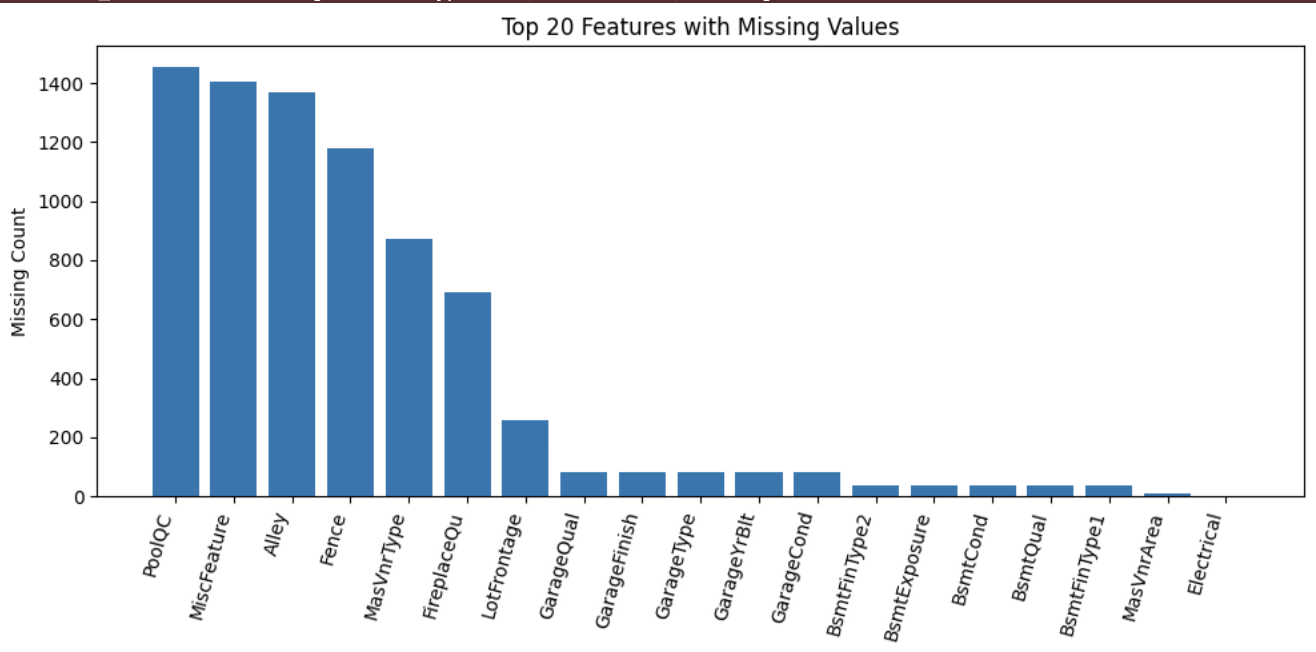
\includegraphics[width=0.8\linewidth]{images/Top_20_Features_with_Missing_Values.png}
    \caption{Top 20 features with the highest number of missing values.}
    \label{fig:missing-values}
\end{figure}

\subsection{Target Distribution and Transformation}
\label{sec:eda-target}

The raw distribution of \texttt{SalePrice} is strongly right-skewed, with a long tail of expensive properties.
This violates the normality assumption underlying many regression models and can cause models to underperform on typical houses or be overly influenced by outliers.

Using the notebook, we visualised the histogram of \texttt{SalePrice} and then the histogram of \(\log(1 + \texttt{SalePrice})\).
These are saved as:

\begin{itemize}[leftmargin=*]
    \item \texttt{images/salePrice\_before\_log1p.png}
    \item \texttt{images/salePrice\_after\_log1p.png}
\end{itemize}

\begin{figure}[h]
    \centering
    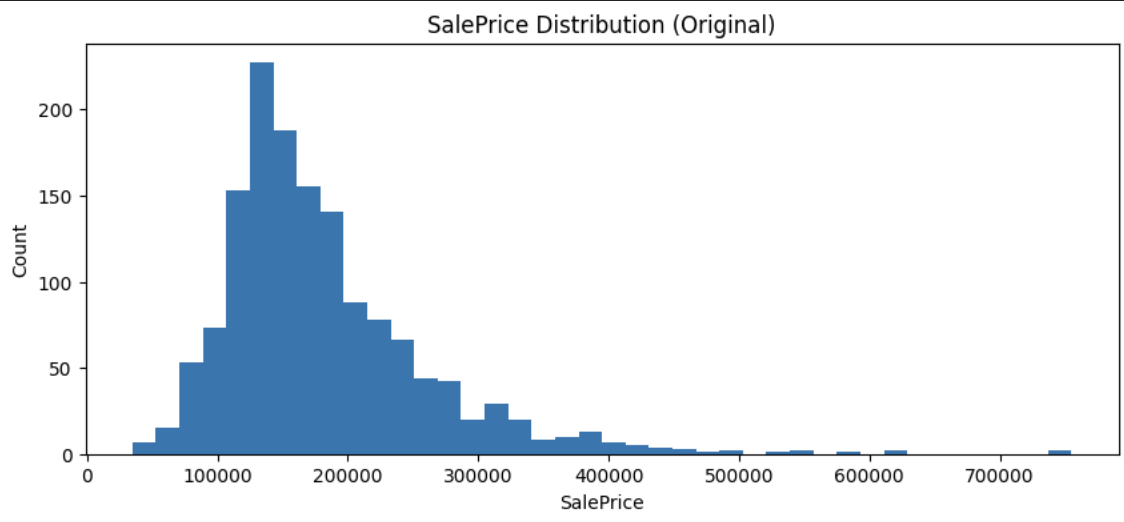
\includegraphics[width=0.47\linewidth]{images/salePrice_before_log1p.png}
    \hfill
    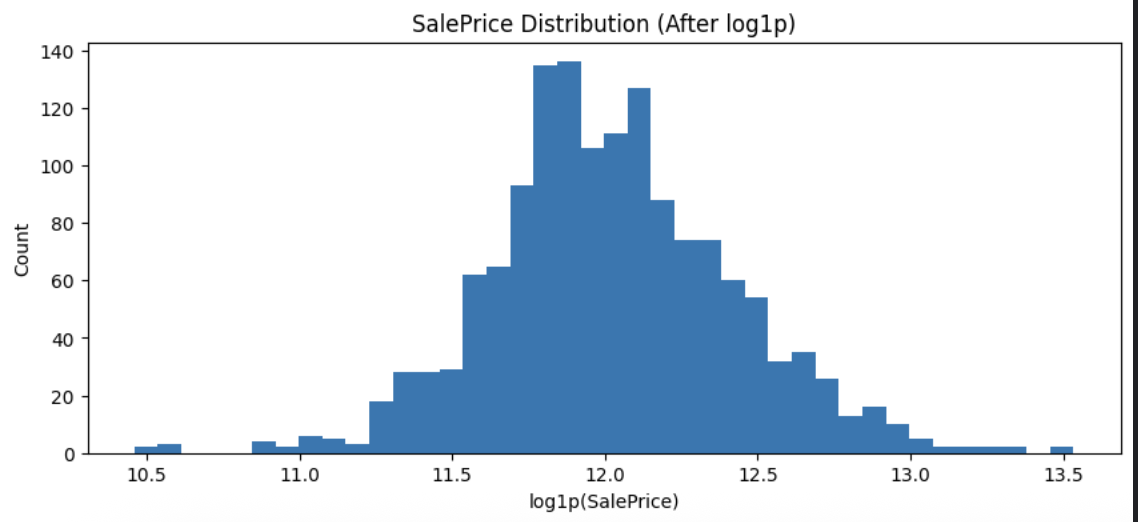
\includegraphics[width=0.47\linewidth]{images/salePrice_after_log1p.png}
    \caption{Distribution of \texttt{SalePrice} before (left) and after (right) \(\log(1 + x)\) transformation.}
    \label{fig:target-transform}
\end{figure}

The log-transformed target is much closer to a symmetric, approximately normal distribution, which stabilises training and improves model fit.

\subsection{Correlation Analysis}

We computed the Pearson correlation between numeric features and the target (in USD) and plotted the 12 most correlated numeric features.
This plot is saved as \texttt{images/Top12\_Numeric\_Features\_Correlation.png}.

Key observations:

\begin{itemize}[leftmargin=*]
    \item \textbf{Overall quality (\texttt{OverallQual})} has one of the strongest positive correlations with \texttt{SalePrice}.
    \item \textbf{Living area (\texttt{GrLivArea})} and \textbf{basement area} (\texttt{TotalBsmtSF}) are also highly correlated.
    \item \textbf{Garage capacity} (\texttt{GarageCars}) and \textbf{year built} (\texttt{YearBuilt}) show meaningful positive correlations.
\end{itemize}

These insights motivated both the choice of input features highlighted in the Streamlit UI and the expectation that a mostly linear model might perform well after appropriate transformations.

\begin{figure}[h]
    \centering
    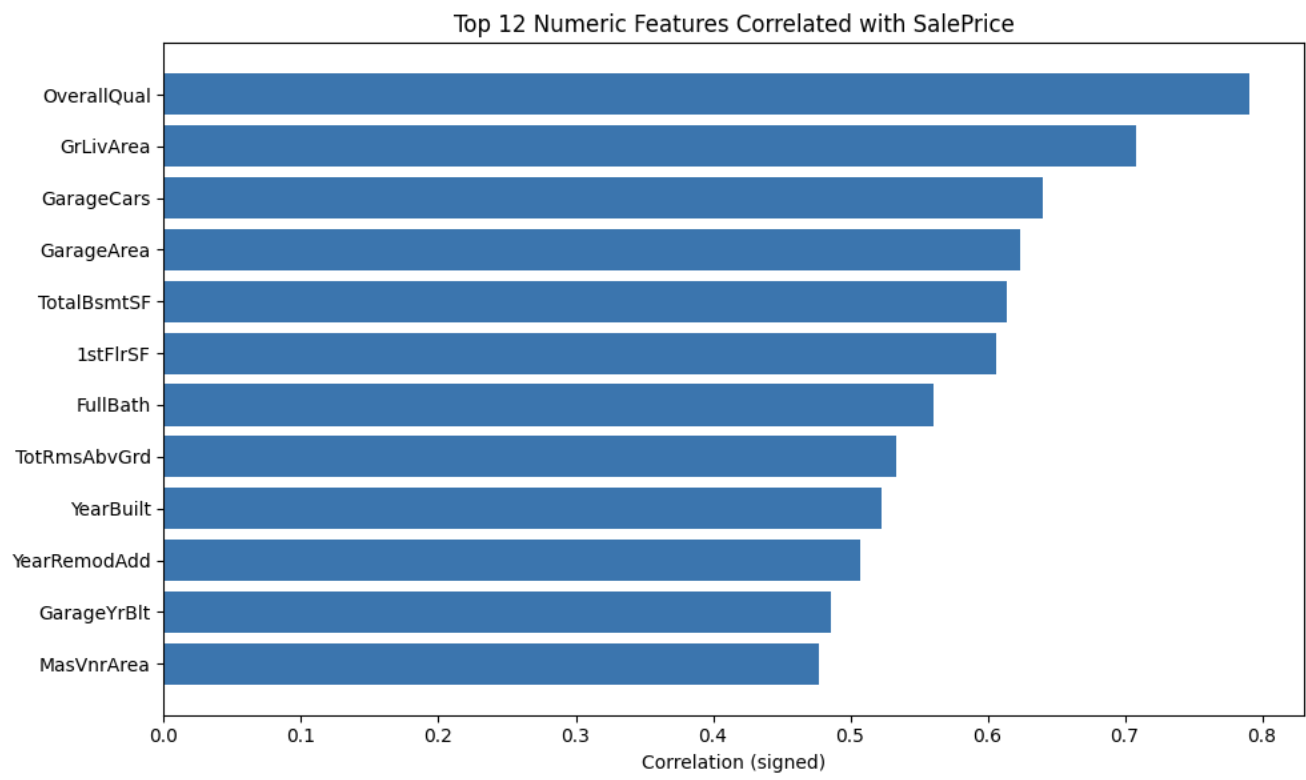
\includegraphics[width=0.8\linewidth]{images/Top12_Numeric_Features_Correlation.png}
    \caption{Top 12 numeric features by absolute correlation with \texttt{SalePrice}.}
\end{figure}

\subsection{Train--Validation Split}

To obtain unbiased estimates of model performance, we split the dataset into training and validation sets:

\begin{itemize}[leftmargin=*]
    \item \textbf{Train:} 80\% of the data.
    \item \textbf{Validation:} 20\% of the data.
    \item \textbf{Random seed:} 42 (for reproducibility).
\end{itemize}

This split results in 1168 training examples and 292 validation examples.
The same split is used for all model comparisons to ensure fairness.

% -------------------------------------------------
% 4. Methodology
% -------------------------------------------------
\section{Methodology}

\subsection{Overall Pipeline Design}

Instead of manually cleaning and transforming features in an ad hoc manner, we use a \textbf{scikit-learn pipeline} based on \texttt{ColumnTransformer} and \texttt{Pipeline} objects.
This design has several advantages:

\begin{itemize}[leftmargin=*]
    \item Training and inference (in the Streamlit app) run the \textbf{exact same} preprocessing steps.
    \item Complex transformations are encapsulated and reproducible.
    \item The final model artifact can be serialised with joblib and loaded directly in production.
\end{itemize}

The high-level flow is:

\begin{enumerate}[leftmargin=*]
    \item Load and clean raw data.
    \item Separate features \(\mathbf{X}\) and target \(y = \texttt{SalePrice}\).
    \item Drop the \texttt{Id} column.
    \item Split into training and validation sets.
    \item Apply \(\log(1 + y)\) transformation to the target for training.
    \item Fit preprocessing + model pipelines on training data.
    \item Evaluate on the validation set, converting predictions back to USD using \(\exp(y_{\log}) - 1\).
    \item Save the final pipeline, target transform flag, and training column names as a joblib artifact.
\end{enumerate}

\subsection{Preprocessing for Numeric Features}

Numeric features are processed through the following steps:

\begin{itemize}[leftmargin=*]
    \item \textbf{Missing value imputation:} Replace missing values with the median of each column using \texttt{SimpleImputer(strategy="median")}. 
    \item \textbf{Scaling (for Linear Regression):} Standardise features to zero mean and unit variance using \texttt{StandardScaler}.
\end{itemize}

For the Random Forest model, scaling is not required, so we only perform median imputation.

\subsection{Preprocessing for Categorical Features}

Categorical features undergo:

\begin{itemize}[leftmargin=*]
    \item \textbf{Most-frequent imputation:} Fill missing values with the most frequent category per column.
    \item \textbf{One-hot encoding:} Convert categorical values into binary indicator columns using \texttt{OneHotEncoder(handle\_unknown="ignore")}.
\end{itemize}

Using \texttt{handle\_unknown="ignore"} ensures that the model can safely process categories that did not appear during training (important in deployment).

\subsection{Target Transformation}

As established in Section~\ref{sec:eda-target}, the target \texttt{SalePrice} is right-skewed.
We therefore train models on:

\[
y_{\log} = \log(1 + \texttt{SalePrice})
\]

At prediction time, we invert this transformation to obtain prices in USD:

\[
\widehat{\texttt{SalePrice}} = \exp(y_{\log}^{\text{pred}}) - 1
\]

This transformation:

\begin{itemize}[leftmargin=*]
    \item Reduces the influence of extreme outliers.
    \item Brings the target distribution closer to normal.
    \item Often improves both MAE and RMSE for regression tasks with heavy-tailed targets.
\end{itemize}

The transformation flag (\texttt{"log1p"}) is stored with the saved artifact so the Streamlit app can consistently apply the inverse transform via \texttt{numpy.expm1}.

\subsection{Baseline Model: Linear Regression}

We first build a baseline using ordinary least squares Linear Regression:

\begin{itemize}[leftmargin=*]
    \item \textbf{Model:} scikit-learn's \texttt{LinearRegression}.
    \item \textbf{Pipeline:}
    \begin{itemize}
        \item Numeric: median imputation + standard scaling.
        \item Categorical: most-frequent imputation + one-hot encoding.
        \item Regressor: Linear Regression trained on \(y_{\log}\).
    \end{itemize}
\end{itemize}

The Linear Regression pipeline is simple, fast, and provides a strong baseline for comparison.

\subsection{Comparison Model: Random Forest Regressor}

To capture potential non-linear relationships and interactions, we also train a Random Forest Regressor:

\begin{itemize}[leftmargin=*]
    \item \textbf{Model:} \texttt{RandomForestRegressor} with:
    \begin{itemize}
        \item \texttt{n\_estimators = 600}
        \item \texttt{random\_state = 42}
        \item \texttt{n\_jobs = -1} (parallel training)
        \item Other parameters set to defaults (e.g.\ \texttt{max\_depth=None}).
    \end{itemize}
    \item \textbf{Pipeline:}
    \begin{itemize}
        \item Numeric: median imputation (no scaling).
        \item Categorical: most-frequent imputation + one-hot encoding.
        \item Regressor: Random Forest trained on \(y_{\log}\).
    \end{itemize}
\end{itemize}

Random Forest can automatically model non-linearities and feature interactions, although at the cost of greater complexity and less interpretability compared to Linear Regression.

\subsection{Model Serialization and Deployment Artifacts}

After training, we save the artifacts using joblib:

\begin{itemize}[leftmargin=*]
    \item \textbf{Pipeline:} The final trained Linear Regression pipeline (preprocessing + model).
    \item \textbf{Target transform flag:} \texttt{"log1p"} to indicate the target was transformed.
    \item \textbf{Training columns:} The list of original feature columns expected by the pipeline.
\end{itemize}

These are stored in a single joblib file (\texttt{model/house\_price\_lr\_pipeline.joblib}) which is loaded by the Streamlit app.

The deployed application uses:

\begin{itemize}[leftmargin=*]
    \item \textbf{\texttt{load\_artifacts}:} Loads the saved pipeline, target transform, and training columns.
    \item \textbf{\texttt{build\_input\_df}:} Constructs a single-row \texttt{pandas.DataFrame} matching the training feature schema.
    \item \textbf{\texttt{predict\_usd}:} Runs the pipeline, applies the inverse transform if required, validates the prediction, and returns a final price in USD.
\end{itemize}

% -------------------------------------------------
% 5. Evaluation
% -------------------------------------------------
\section{Evaluation}

\subsection{Metrics}

We evaluate regression performance on the validation set using:

\begin{itemize}[leftmargin=*]
    \item \textbf{MAE (Mean Absolute Error):}
    \[
    \text{MAE} = \frac{1}{n} \sum_{i=1}^n \left| y_i - \hat{y}_i \right|
    \]
    Measures the average absolute deviation in USD.
    \item \textbf{RMSE (Root Mean Squared Error):}
    \[
    \text{RMSE} = \sqrt{\frac{1}{n} \sum_{i=1}^n \left( y_i - \hat{y}_i \right)^2}
    \]
    Penalises larger errors more heavily than MAE.
    \item \textbf{R\textsuperscript{2} (Coefficient of Determination):}
    \[
    R^2 = 1 - \frac{\sum_i (y_i - \hat{y}_i)^2}{\sum_i (y_i - \bar{y})^2}
    \]
    Measures the proportion of variance in the target explained by the model.
\end{itemize}

All metrics are reported in the original price space (USD), after inverting the log-transform.

\subsection{Quantitative Results}

Table~\ref{tab:metrics} summarises the performance of both models on the validation set.

\begin{table}[h]
    \centering
    \caption{Validation performance of Linear Regression and Random Forest models.}
    \label{tab:metrics}
    \begin{tabular}{l
                    S[table-format=5.0]
                    S[table-format=5.0]
                    S[table-format=1.4]}
        \toprule
        \textbf{Model} & \textbf{MAE (USD)} & \textbf{RMSE (USD)} & \textbf{R\textsuperscript{2}} \\
        \midrule
        Linear Regression (log target) & 14899 & 22740 & 0.9326 \\
        Random Forest (log target)     & 17495 & 30153 & 0.8815 \\
        \bottomrule
    \end{tabular}
\end{table}

\subsection{Interpretation}

Despite being simpler, the Linear Regression model:

\begin{itemize}[leftmargin=*]
    \item Achieves a \textbf{lower MAE and RMSE} compared to the Random Forest.
    \item Explains a \textbf{higher proportion of variance} in prices (R\textsuperscript{2}~\(\approx 0.93\) vs.~0.88).
\end{itemize}

These results suggest that, after appropriate preprocessing and log-transforming the target, the relationship between the selected features and \texttt{SalePrice} is largely linear.
The more complex Random Forest model underperforms, likely because it overfits some noise and does not benefit enough from modelling non-linearities.

\subsection{Model Selection}

Based on the validation metrics and practical concerns (speed, interpretability, and ease of deployment), we select the \textbf{Linear Regression (log target)} pipeline as the final model for deployment.

% -------------------------------------------------
% 6. Optimization
% -------------------------------------------------
\section{Optimization and Design Choices}

This section summarises the key optimisation steps taken to improve model performance and deployment readiness.

\subsection{Data Cleaning and Preprocessing}

\begin{itemize}[leftmargin=*]
    \item \textbf{Identifier removal:} The \texttt{Id} column, which does not carry predictive information, was removed.
    \item \textbf{Missing value handling:} We used median imputation for numeric columns and most-frequent imputation for categorical columns.
    \item \textbf{Consistent pipeline:} All preprocessing was encapsulated in scikit-learn pipelines, ensuring that training and inference apply identical transformations.
\end{itemize}

\subsection{Target Transformation}

Using a \(\log(1 + x)\) target transformation improved the stability of training and reduced the influence of extremely expensive properties.
This was one of the most impactful optimisations and directly improved both MAE and R\textsuperscript{2}.

\subsection{Model Architecture and Hyperparameters}

\begin{itemize}[leftmargin=*]
    \item \textbf{Baseline vs.\ complex models:} We intentionally kept a simple, well-regularised Linear Regression baseline for comparison.
    \item \textbf{Random Forest tuning:} 
    \begin{itemize}
        \item Increased the number of trees (\texttt{n\_estimators = 600}) to stabilise the ensemble.
        \item Allowed deep trees to capture potentially complex patterns.
    \end{itemize}
    While this improved the robustness of the Random Forest relative to naive defaults, it still did not surpass Linear Regression on the validation metrics.
\end{itemize}

\subsection{Feature Selection and UI Design}

From EDA and domain reasoning, we identified a set of high-impact and user-friendly features to expose in the Streamlit app:

\begin{itemize}[leftmargin=*]
    \item Overall quality (\texttt{OverallQual})
    \item Living area (\texttt{GrLivArea})
    \item Garage capacity (\texttt{GarageCars})
    \item Basement area (\texttt{TotalBsmtSF})
    \item Year built (\texttt{YearBuilt})
    \item Number of full bathrooms (\texttt{FullBath})
    \item Number of fireplaces (\texttt{Fireplaces})
    \item Lot area (\texttt{LotArea})
\end{itemize}

These features strike a balance between:

\begin{itemize}[leftmargin=*]
    \item \textbf{Predictive power} (high correlation with price).
    \item \textbf{User interpretability} in the UI.
    \item \textbf{Simplicity} of input, avoiding overwhelming the user with dozens of sliders and text fields.
\end{itemize}

\subsection{Deployment Optimizations}

\begin{itemize}[leftmargin=*]
    \item \textbf{Single artifact:} Packaging the entire preprocessing + model pipeline into one joblib file simplifies deployment and reduces the risk of mismatched transformations.
    \item \textbf{Version pinning:} We pinned critical library versions in \texttt{requirements.txt} to ensure compatibility with the saved artifact. For example:
    \begin{itemize}
        \item scikit-learn~1.6.1
        \item joblib~1.5.3
        \item numpy~2.0.2
        \item pandas~2.3.3
    \end{itemize}
    \item \textbf{Robust prediction function:} The prediction wrapper in the app checks for invalid (non-finite or negative) outputs and raises a clear error if encountered.
\end{itemize}

% -------------------------------------------------
% 7. Streamlit Application
% -------------------------------------------------
\section{Streamlit Application}

Although not strictly required by the rubric, deployment is an important aspect of the project.

\subsection{User Interface}

The Streamlit app provides:

\begin{itemize}[leftmargin=*]
    \item A \textbf{prediction card} showing the latest estimated price in USD with nice formatting.
    \item A set of \textbf{sliders and number inputs} for the key features listed in the previous section.
    \item A \textbf{prediction history line chart} plotting previous predictions over runs.
    \item A \textbf{history table} summarising each run, including the chosen feature values and the corresponding predicted price.
\end{itemize}

The UI is styled to be clean and modern, and it operates without a sidebar, focusing the user’s attention on the main interactive elements.

\subsection{Prediction Workflow}

For each prediction:

\begin{enumerate}[leftmargin=*]
    \item The app collects user inputs for the selected features.
    \item \texttt{build\_input\_df} creates a single-row DataFrame with the same columns as the training data and fills provided values.
    \item The loaded pipeline transforms the input and produces a log-space prediction.
    \item \texttt{predict\_usd} applies \texttt{expm1} if the target transform flag is set to \texttt{"log1p"}.
    \item The resulting price is validated (finite, non-negative) and presented to the user.
    \item The prediction is appended to an in-memory history list, which updates the chart and table.
\end{enumerate}

This design ensures that the deployed system closely mirrors the training environment and that predictions remain consistent and reproducible.

% -------------------------------------------------
% 8. Team Contribution
% -------------------------------------------------
\section{Team Contribution}

The project was a collaborative effort. Each team member had clearly defined responsibilities, which are summarised below.

\subsection*{Kavya Katal}

\begin{itemize}[leftmargin=*]
    \item Led \textbf{model training} and experimentation in the Jupyter notebooks.
    \item Designed and implemented the \textbf{preprocessing pipelines} using \texttt{ColumnTransformer} and \texttt{Pipeline}.
    \item Trained and evaluated the \textbf{Linear Regression} and \textbf{Random Forest} models.
    \item Contributed to the \textbf{technical report} and documentation of the modelling decisions.
\end{itemize}

\subsection*{Aabir Sarkar}

\begin{itemize}[leftmargin=*]
    \item Handled \textbf{data cleaning and preprocessing}, including handling missing values, column type checks, and dataset sanity validation.
    \item Implemented the \textbf{Streamlit application} logic, including loading the saved artifacts, building input DataFrames, and running predictions.
    \item Wrote and refined the \textbf{LaTeX report}, integrating results from the notebook and codebase.
    \item Created and organised supporting project assets (e.g., figures and configuration files).
\end{itemize}

\subsection*{Kushagra Maheswari}

\begin{itemize}[leftmargin=*]
    \item Responsible for \textbf{dataset sourcing}, ensuring the correct Ames Housing dataset was obtained and integrated into the project.
    \item Created the \textbf{demo video} showcasing the model and the Streamlit app in action.
    \item Helped verify that the user interface behaved correctly for different input configurations.
\end{itemize}

\subsection*{Pratyush Chouksey}

\begin{itemize}[leftmargin=*]
    \item Contributed to \textbf{dataset sourcing} and validation of the raw data.
    \item Assisted in writing parts of the \textbf{project report}, especially sections related to data description and EDA.
    \item Helped cross-check the consistency between the notebook results and the deployed model.
\end{itemize}

% -------------------------------------------------
% 9. Conclusion
% -------------------------------------------------
\section{Conclusion}

In this project, we built a complete property price prediction system, from data preprocessing and model training to deployment in a user-friendly Streamlit interface.
Through systematic EDA, we identified key features and addressed data quality issues.
Using scikit-learn pipelines with a log-transformed target, we compared a baseline Linear Regression model with a Random Forest Regressor and empirically found that the simpler Linear Regression model achieved superior performance (MAE \(\approx\)\,\$14{,}899, R\textsuperscript{2} \(\approx\)\,0.93).

The final deployed model provides fast, stable estimates of house prices and demonstrates the importance of robust preprocessing, careful model selection, and end-to-end reproducibility.
Future work could explore additional models (e.g., Gradient Boosting, XGBoost), richer feature engineering, uncertainty quantification, and integration of explainability techniques such as SHAP values.

\end{document}